A data scientist working on housing price prediction is trying to understand their trained classifier's decision patterns for specific predictions. They have developed a custom Random Forest model on the California Housing dataset and need to explain predictions for stakeholder communication. Since they were already working in the Jupyter Notebook environment, the data scientist opts to use the interface through that tool, which allows integration of their pre-trained classifier directly into the explanation workflow.

\subsection{Dataset Preparation and Model Configuration}

The data scientist begins by preparing the California Housing dataset for their analysis task. The original dataset contains median house values as continuous targets. They transform this regression problem into a five-class classification task by dividing the target into equal-frequency percentile bands. Each band represents twenty percent of the data distribution: percentile\_0 (lowest prices, \$15,000-\$107,200), percentile\_1 (\$107,200-\$157,300), percentile\_2 (\$157,300-\$209,400), percentile\_3 (\$209,400-\$290,000), and percentile\_4 (highest prices, \$290,000-\$500,000).

This discretization choice serves multiple analytical purposes. It converts a complex regression problem into interpretable price categories that align with real estate market segments. The equal-frequency binning ensures balanced class representation across the dataset, avoiding issues with sparse high-value regions. The resulting five-class structure provides sufficient granularity to distinguish meaningful price tiers while maintaining interpretability.

The dataset features eight attributes characterizing housing blocks in California: median income (MedInc), house age (HouseAge), average rooms (AveRooms), average bedrooms (AveBedrms), population, average occupancy (AveOccup), latitude, and longitude. The data scientist recognizes that geographic coordinates (latitude and longitude) carry particular importance in housing price prediction, as location fundamentally determines property values in real estate markets.

They construct a preprocessing pipeline using scikit-learn's ColumnTransformer, applying StandardScaler to all numeric features. Without standardization, features with larger numeric ranges would disproportionately influence neighborhood generation.

For the classifier, the data scientist selects Random Forest and performs systematic hyperparameter optimization. They conduct grid search over 1,152 parameter combinations using ten percent of the data to identify optimal hyperparameters efficiently. The search evaluates n\_estimators (50, 100, 200, 300), max\_depth (10, 20, 30, None), min\_samples\_split (2, 5, 10), min\_samples\_leaf (1, 2, 4), max\_features (sqrt, log2), and bootstrap options (True, False). Ten-fold cross-validation on the sample ensures robust parameter selection.

The optimization process identifies the following configuration: 200 trees, maximum depth 30, minimum samples split 5, minimum samples leaf 1, sqrt max features, and bootstrap enabled. The data scientist trains the final model on the complete dataset using these parameters with a 70-30 train-test split. Cross-validation on the full training set yields 0.8156 accuracy, while the held-out test set achieves 0.8098 accuracy. The Random Forest produces well-calibrated predictions across all five price percentile classes, with particularly strong performance in the extreme percentiles (percentile\_0 and percentile\_4) where feature patterns prove most distinctive.

\subsection{Instance Selection and Interface Initialization}

The data scientist selects an instance for explanation: a property with median income \$830,140, house age 21 years, 6.24 average rooms, 0.97 average bedrooms, population 2,401, average occupancy 2.11, located at latitude 37.86 and longitude -122.22. The Random Forest predicts this instance as percentile\_4, the highest price category. These coordinates place the property in the East Bay region of the San Francisco Bay Area, a location where high property values align with expectations given the elevated median income.

They initialize the Jupyter interface by creating a \texttt{TabularGeneticGeneratorLore} object, passing their trained classifier (wrapped as a black-box predictor) and the dataset descriptor. The data scientist calls the \texttt{interactive\_explanation} method with the selected instance, setting \texttt{inJupyter=False} to launch the full browser-based interface rather than an embedded notebook view. This choice provides access to the complete visualization system with full interaction capabilities.

The interface opens in the browser, bypassing the dataset selection, classifier selection, and model training sections since the classifier and instance were already provided. The interface proceeds directly to the explanation parameter configuration, where the data scientist can adjust neighborhood size, dimensionality reduction settings, and visualization preferences.

\subsection{Initial Explanation with Default Parameters}

The data scientist begins their analysis with the default neighborhood size of 500 synthetic instances. They accept the default UMAP and PCA dimensionality reduction parameters. They initiate explanation generation by clicking the \texttt{Explain!} button.

The system generates 500 synthetic neighbors around the target instance using the genetic algorithm, trains the surrogate decision tree on this neighborhood, and extracts both the factual and counterfactual rules. The visualization components render simultaneously: the 2D scatter plot showing the synthetic neighborhood projected via UMAP, shown in Figure \ref{fig:ds_scatter_umap_500}, and the tree visualization of the surrogate model, shown in Figure \ref{fig:ds_Blocks_500}.

The data scientist examines the UMAP projection first. The visualization reveals distinct spatial clusters corresponding to different predicted price percentiles. A dense cluster of percentile\_4 instances (\#fee090) appears in the middle right quadrant, including the explained instance. Scattered percentile\_3 instances (\#41b6c4) form smaller groups, some intermixed with percentile\_4 instances along cluster boundaries, others forming an isolated cluster in the bottom left. The spatial separation between percentile\_4 and lower percentiles appears relatively clear, though some percentile\_3 instances lie close to the percentile\_4 cluster boundary.

The data scientist notices that the synthetic neighborhood exhibits uneven class distribution. The majority of generated instances receive percentile\_4 predictions, matching the explained instance's class. Fewer percentile\_3 instances appear, and percentile\_0, percentile\_1, and percentile\_2 instances are nearly absent from this particular neighborhood generation. This absence reflects the genetic algorithm's characteristic behavior: it focuses exploration on the local decision space around the explained instance. Since the explained instance belongs to percentile\_4 with a confident prediction, the algorithm generates synthetic neighbors primarily within and immediately adjacent to this high-value region. Exploring distant feature value combinations corresponding to percentile\_0, percentile\_1, or percentile\_2 would require traversing substantial feature space distances from the explained instance. The genetic algorithm's fitness function prioritizes generating instances that maintain proximity to the target instance while exploring local decision boundaries, resulting in concentrated sampling within the percentile\_4 region and its immediate neighbors.

They switch to the PCA projection, shown in Figure \ref{fig:ds_scatter_pca_500}, to examine decision boundaries more directly. The PCA method enables Voronoi tessellation-based boundary visualization, which approximates the classifier's decision regions using a grid of test points.

\begin{figure}[ht]
\centering
\begin{subfigure}[c]{0.48\textwidth}
\centering
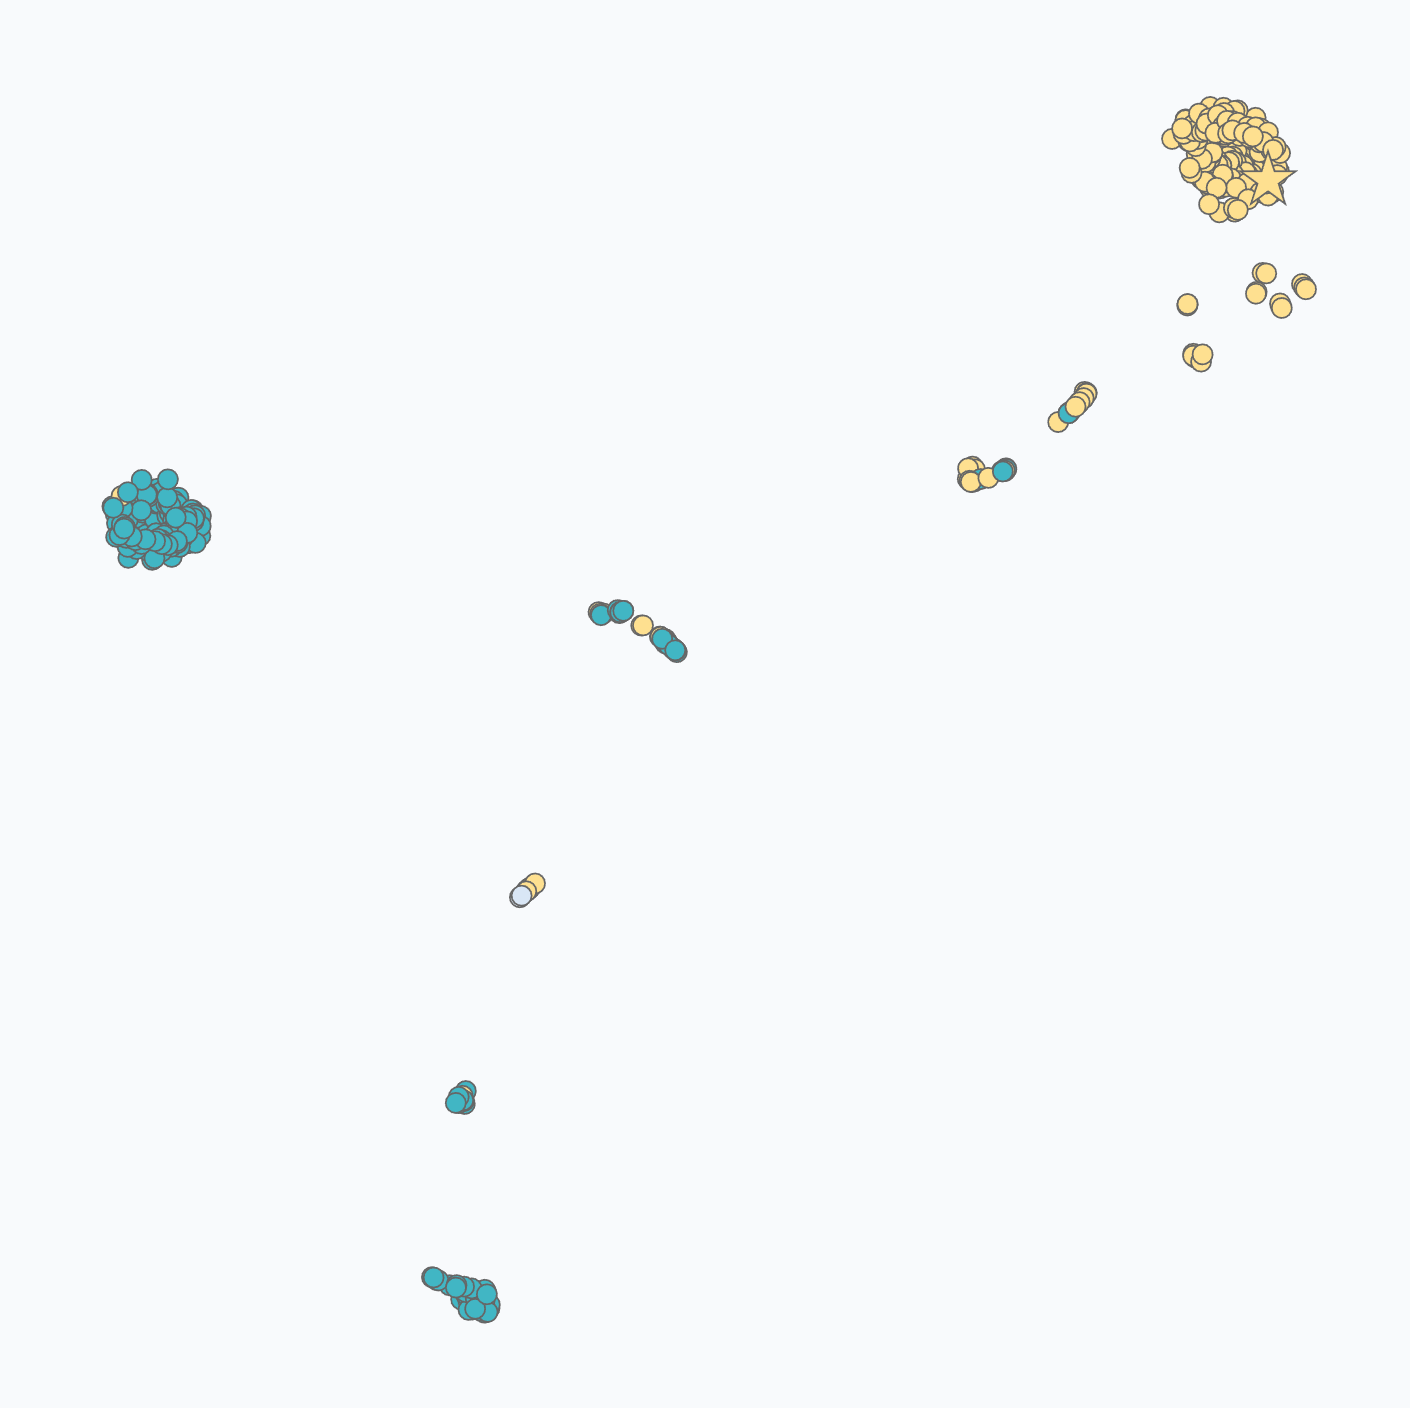
\includegraphics[width=\textwidth]{images/ds_scatter_umap_500.png}
\caption{UMAP projection}
\label{fig:ds_scatter_umap_500}
\end{subfigure}
\hfill
\begin{subfigure}[c]{0.48\textwidth}
\centering
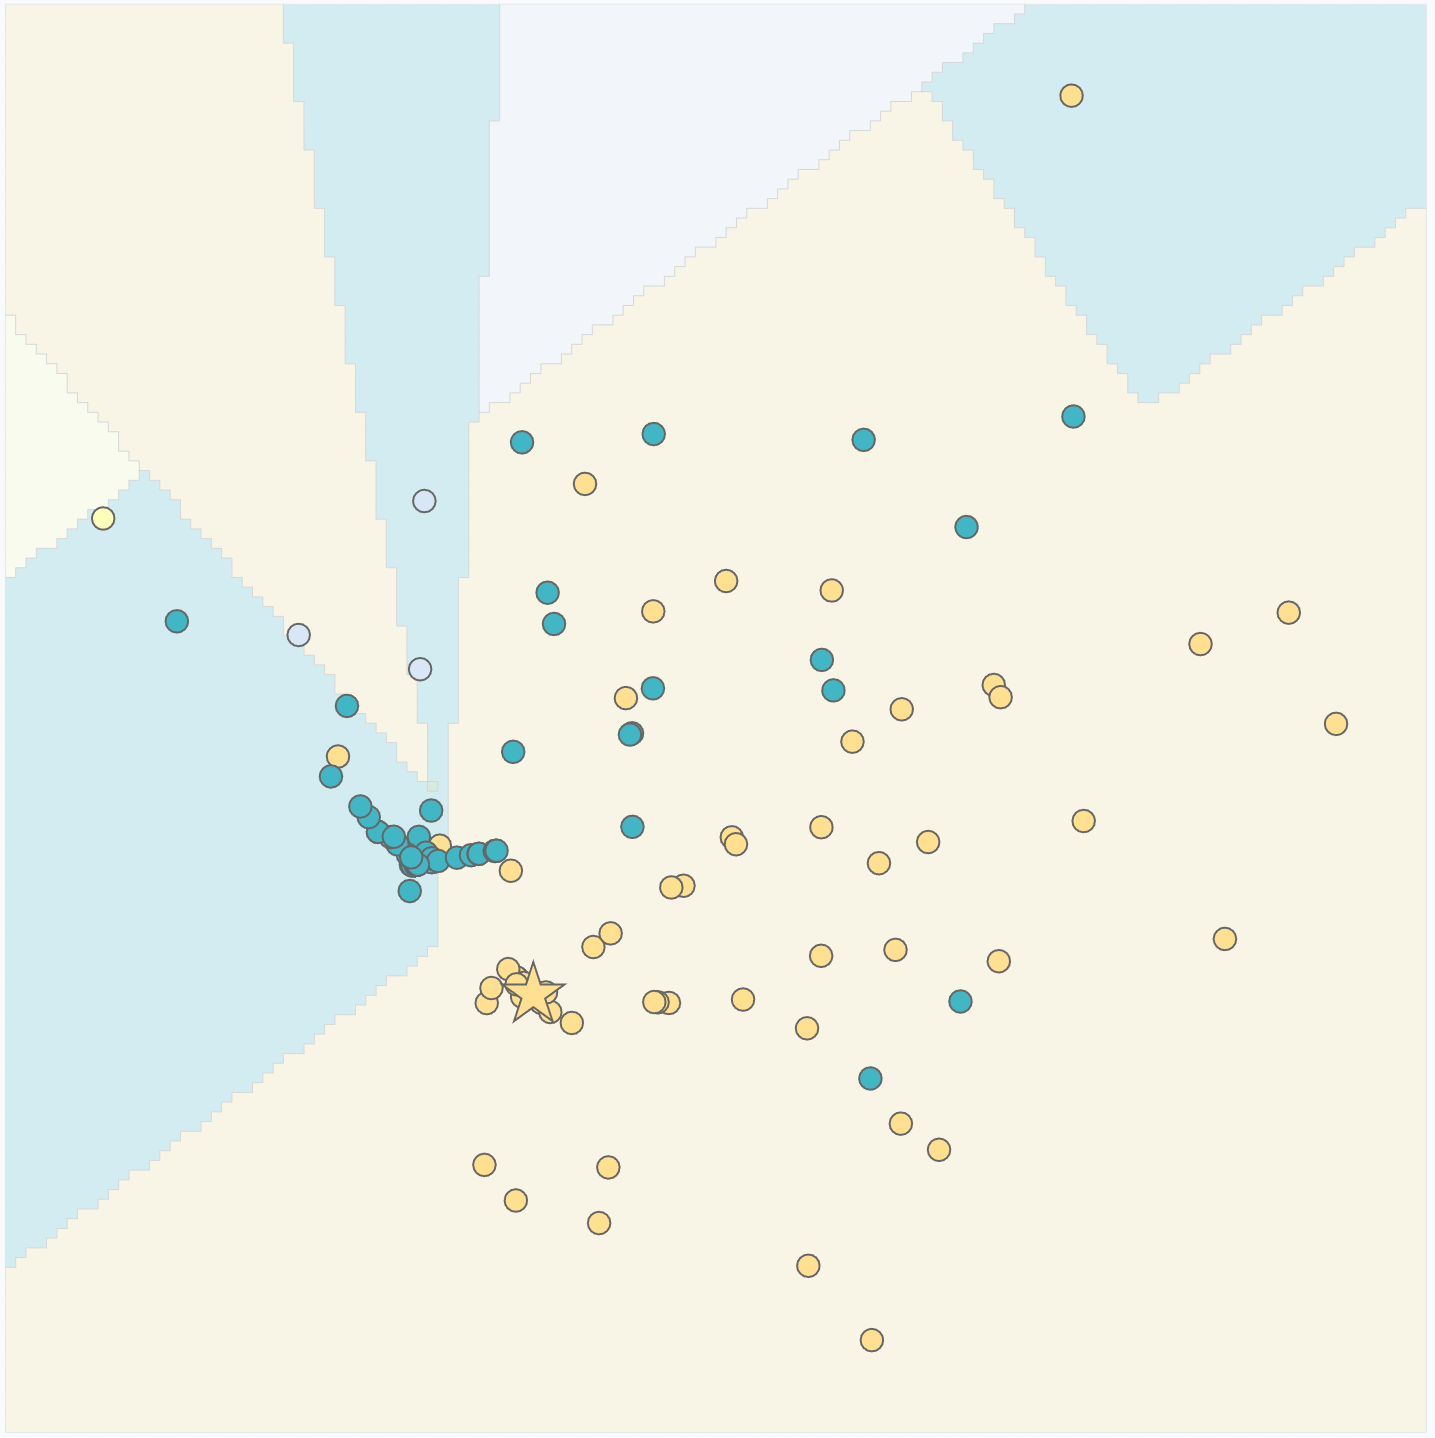
\includegraphics[width=\textwidth]{images/ds_scatter_pca_500.png}
\caption{PCA projection with decision boundaries}
\label{fig:ds_scatter_pca_500}
\end{subfigure}
\caption{Spatial neighborhood visualizations for 500-instance synthetic neighborhood: UMAP projection showing cluster structure (a) and PCA projection with Voronoi tessellation-based decision boundary visualization (b)}
\label{fig:scatter_500_comparison}
\end{figure}

The PCA projection displays decision boundaries rendered as colored background regions. The percentile\_4 region (light \#fee090) dominates the visualization space, occupying most of the bottom right and central portions. A percentile\_3 region (light \#41b6c4) appears in the middle left quadrant. The explained instance (star marker) sits within the percentile\_4 region. The boundary visualization confirms the classifier's confident prediction for this instance. The nearest boundary lies several principal component units away, suggesting that substantial feature modifications would be required to alter the prediction.

\subsection{Surrogate Model Analysis and Rule Extraction}

The data scientist examines the surrogate model to understand the extracted rules. They select the Rule and Counterfactual Rules Centered tree visualization, which positions the explained instance's path at the bottom for easy identification.

Figure \ref{fig:ds_Blocks_500} displays the decision tree structure. The root node splits on MedInc. The explained instance follows the true branch (MedInc $> 7.2$), leading directly to a leaf node predicting percentile\_4. This factual rule is very simple: "If MedInc $> 7.2$, then predict percentile\_4." The single-condition rule indicates that median income above \$720,000 serves as the primary determinant for high-value property classification in this local decision region.

\begin{figure}[ht]
\centering
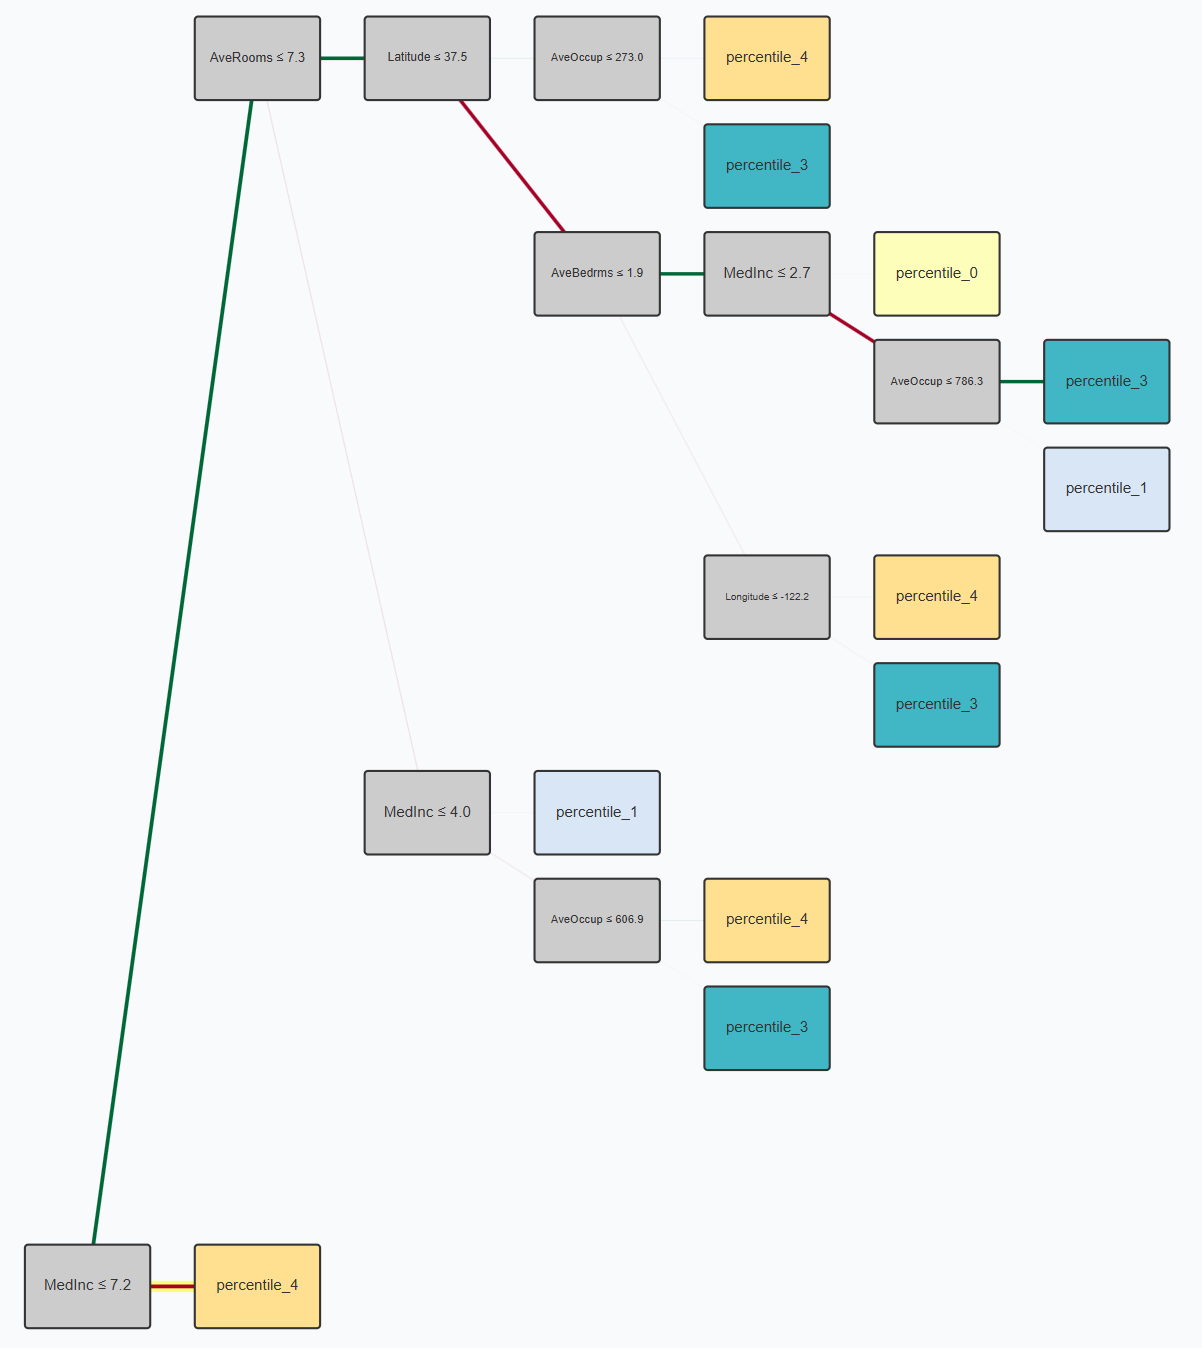
\includegraphics[width=0.5\textwidth]{images/ds_Blocks_500.png}
\caption{Rule and Counterfactual Rules Centered visualization of surrogate model trained on 500-instance neighborhood, showing simple tree structure with factual rule path (MedInc $> 7.2 \rightarrow$ percentile\_4) at bottom and counterfactual path to percentile\_3}
\label{fig:ds_Blocks_500}
\end{figure}

The simplicity of this factual rule provides immediate insight into the classifier's behavior. Properties with median household incomes exceeding \$720,000 receive confident percentile\_4 predictions regardless of other feature values. This threshold aligns with real estate market understanding: neighborhoods with such high median incomes typically command premium property prices. However, the data scientist recognizes that this single-split rule, while interpretable, may be oversimplifying the decision boundary. The rule captures the dominant pattern but potentially obscures secondary factors that influence predictions for edge cases.

The surrogate model also reveals counterfactual rules indicating alternative prediction outcomes. The meaningful counterfactual rule extracted by the explainability method follows the false branch from the root: MedInc $\leq 7.2 \rightarrow$ AveRooms $\leq 7.3 \rightarrow$ Latitude $> 37.5 \rightarrow$ AveBedrms $\leq 1.9 \rightarrow$ MedInc $> 2.7 \rightarrow$ AveOccup $\leq 786.3 \rightarrow$ percentile\_3. This counterfactual rule specifies the conditions under which the classifier predicts percentile\_3 rather than percentile\_4. The rule reveals a hierarchical decision structure: first, median income must fall below \$720,000; then, geographic location (latitude above 37.5°, corresponding to Bay Area regions) combined with moderate occupancy patterns and income above \$270,000 leads to percentile\_3 predictions.

The counterfactual rule provides actionable insight. To shift a prediction from percentile\_4 to percentile\_3, the primary change involves reducing median income below the \$720,000 threshold. However, the subsequent conditions indicate that even with lower income, properties maintain relatively high value (percentile\_3 rather than lower percentiles) when located in premium geographic areas (Latitude $> 37.5$) with reasonable occupancy characteristics. This pattern reflects the real estate principle that location preserves value even when income indicators decline.

The data scientist observes that only one meaningful counterfactual rule emerges from the 500-instance neighborhood. The tree structure shows relatively few alternative paths, with most instances following either the direct percentile\_4 path or the single percentile\_3 counterfactual path. This limited counterfactual diversity suggests that the 500-instance neighborhood may not fully characterize the decision space, particularly for predictions substantially different from percentile\_4.

At this stage, the data scientist recognizes the value of the visual interface compared to the textual rule representations described in Section \ref{sec:lore_sa}. The tree visualization immediately reveals the hierarchical rule structure through spatial arrangement. Following the explained instance's path from root to leaf requires simple visual scanning rather than parsing nested logical conditions. The counterfactual rule, while complex with six conditions, becomes more easily comprehensible through the visual path representation.

\subsection{Recognizing Need for Expanded Analysis}

As previously said, while the data scientist explored the tree structure and examined the individual neighborhood instances, they recognize a potential limitation in the current analysis. They reason that increasing the neighborhood size should generate a more comprehensive sample of the local decision space, potentially uncovering additional counterfactual patterns and providing more robust rule extraction. A larger neighborhood may reveal how the classifier handles edge cases near decision boundaries and may produce additional counterfactual rules or refine the existing rules with more detailed conditions.

The data scientist decides to regenerate the explanation with a substantially larger neighborhood. They select 3,000 instances as the new neighborhood size, a number that should provide adequate representation of alternative decision paths while remaining computationally tractable.

\subsection{Regenerating Explanation with Expanded Neighborhood}

The data scientist returns to the parameter configuration interface and modifies the neighborhood size field from 500 to 3000. They retain all other settings to enable direct comparison with the previous results. They click the \texttt{Explain!} button to initiate the new explanation generation. The computational time increases proportionally with the neighborhood size, as the genetic algorithm must generate and evaluate six times as many synthetic instances, and the decision tree training operates on a larger dataset.

When the visualizations appear, the data scientist immediately observes notable differences from the 500-instance case. The UMAP projection, shown in Figure \ref{fig:ds_scatter_umap_3000}, displays substantially increased instance density across all regions of the plot, especially regarding the decision boundary between percentile\_3 and percentile\_4.

The expanded neighborhood reveals a more nuanced class distribution. While percentile\_4 instances still dominate (as expected given the explained instance's confident classification), the data scientist now observes substantially more percentile\_3 instances interspersed throughout the visualization. The cluster arrangement remains similar to the 500-instance case, but the increased density provides finer-grained characterization of the transition zones. In fact, the new extracted rule is more complex but the root split is constant with the previous explanation. The new extracted rule is the following: $\text{MedInc} > 7.4 \rightarrow \text{Latitude} \leq 41.5 \rightarrow \text{MedInc} \leq 12.6 \rightarrow \text{Population} \leq 18771.9 \rightarrow \text{percentile}_4$.

The increased neighborhood size provides better characterization of the transition zones between classes. The data scientist notices gradual transitions from percentile\_4 to percentile\_3 regions, with intermediate instances forming visible gradients in the UMAP projection. This continuous representation helps them understand how the classifier's confidence degrades as feature values shift away from the explained instance's configuration.

\begin{figure}[ht]
\centering
\begin{subfigure}[c]{0.48\textwidth}
\centering
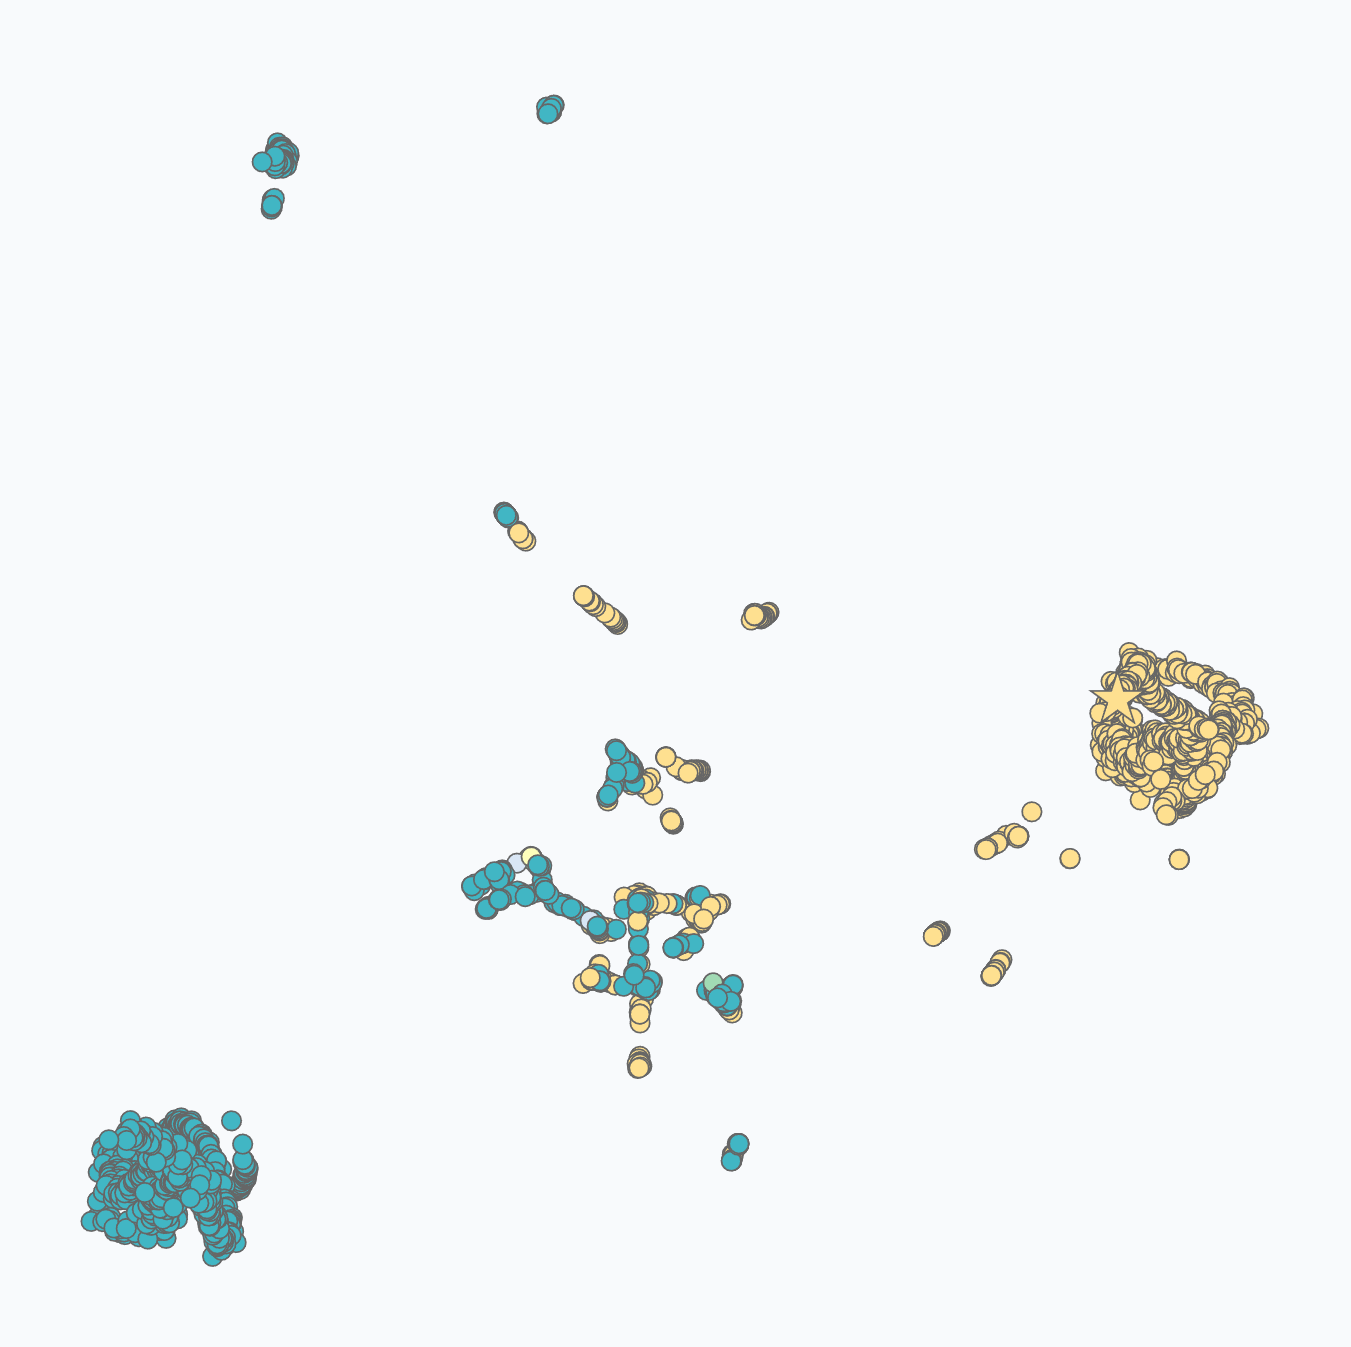
\includegraphics[width=\textwidth]{images/ds_scatter_umap_3000.png}
\caption{UMAP projection}
\label{fig:ds_scatter_umap_3000}
\end{subfigure}
\hfill
\begin{subfigure}[c]{0.48\textwidth}
\centering
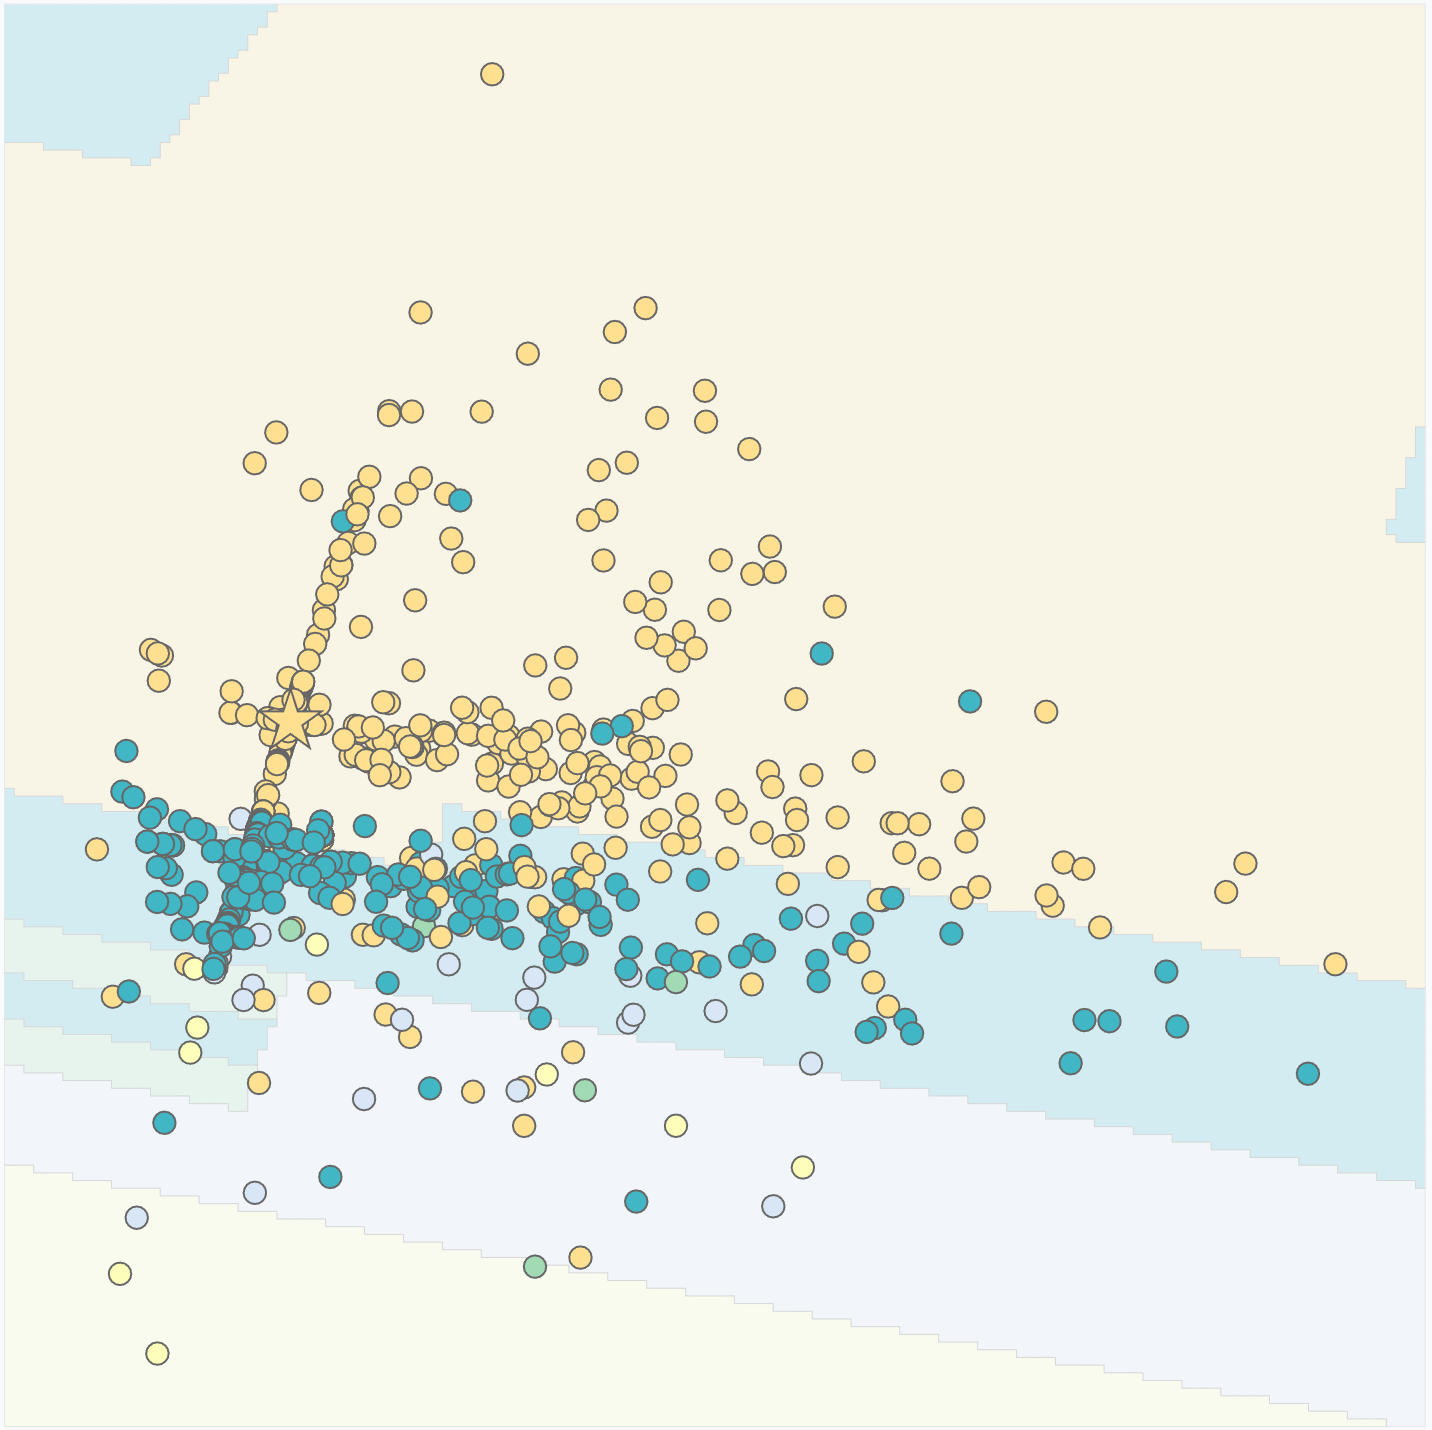
\includegraphics[width=\textwidth]{images/ds_scatter_pca_3000.png}
\caption{PCA projection with decision boundaries}
\label{fig:ds_scatter_pca_3000}
\end{subfigure}
\caption{Spatial neighborhood visualizations for 3000-instance synthetic neighborhood: UMAP projection showing increased density and clearer transition zones (a) and PCA projection revealing presence of all five price percentile classes with band-like decision regions (b)}
\label{fig:scatter_3000_comparison}
\end{figure}

The data scientist switches to the PCA projection to examine how the expanded neighborhood affects decision boundary visualization. Figure \ref{fig:ds_scatter_pca_3000} shows the result.

The PCA boundary visualization with 3,000 instances displays decision region geometry similar in overall structure to the 500-instance case. The percentile\_4 region still occupies the majority of the space, but the data scientist now observes a distinct percentile\_3 region. The class boundaries appear to split the decision space into bands where each class occupies its own region, especially evident for the percentile\_3, percentile\_1, and percentile\_0 classes which form roughly parallel strips.

More significantly, the visualization now reveals clearer regions corresponding to percentile\_2, percentile\_1, and percentile\_0 predictions. These regions, especially the percentile\_2 region, occupy small spaces. Their presence confirms that the expanded neighborhood successfully generated synthetic instances exploring more distant regions of the feature space, uncovering decision patterns that were not relevant in the smaller neighborhood's focused local exploration.

The data scientist examines the surrogate tree trained on the 3,000-instance neighborhood, shown in Figure \ref{fig:ds_tree_3000}. The tree exhibits increased depth and structural complexity compared to the 500-instance tree. The root split still occurs on MedInc, but the threshold shifts slightly to 7.4 (from 7.2 in the smaller neighborhood). The factual rule path now extends through multiple splits, incorporating secondary conditions on Latitude, a second MedInc constraint establishing an upper bound, and Population. This refined rule structure provides more detailed characterization of the decision logic while maintaining consistency with the simpler 500-instance rule in its fundamental pattern.

\begin{figure}[ht]
\centering
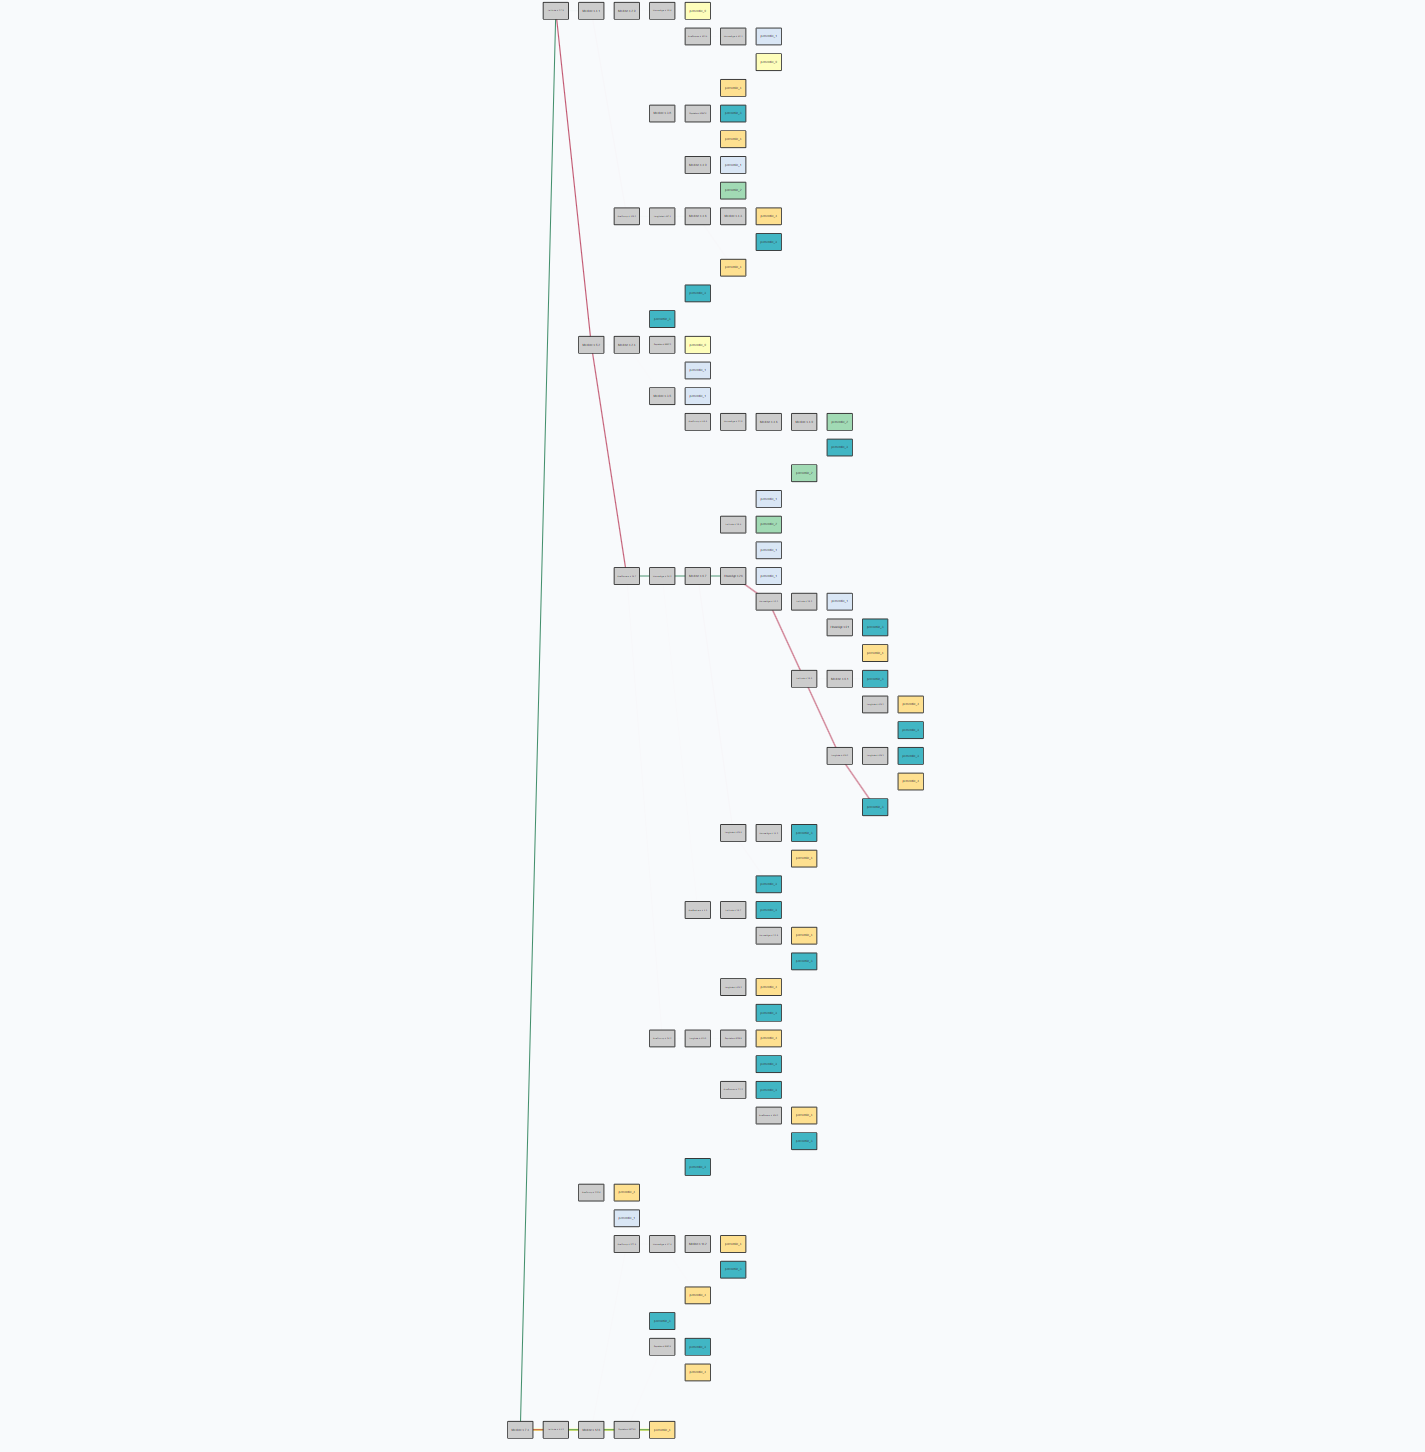
\includegraphics[width=0.7\textwidth]{images/ds_tree_3000.png}
\caption{Rule and Counterfactual Rules Centered visualization of surrogate model trained on 3000-instance neighborhood, showing increased tree depth and refined factual rule with dual MedInc conditions bounding the typical high-value income range}
\label{fig:ds_tree_3000}
\end{figure}

\subsection{Detailed Interaction-Driven Exploration}

\begin{figure}[p]
    \centering
    \begin{subfigure}[c]{0.48\textwidth}
        \centering
        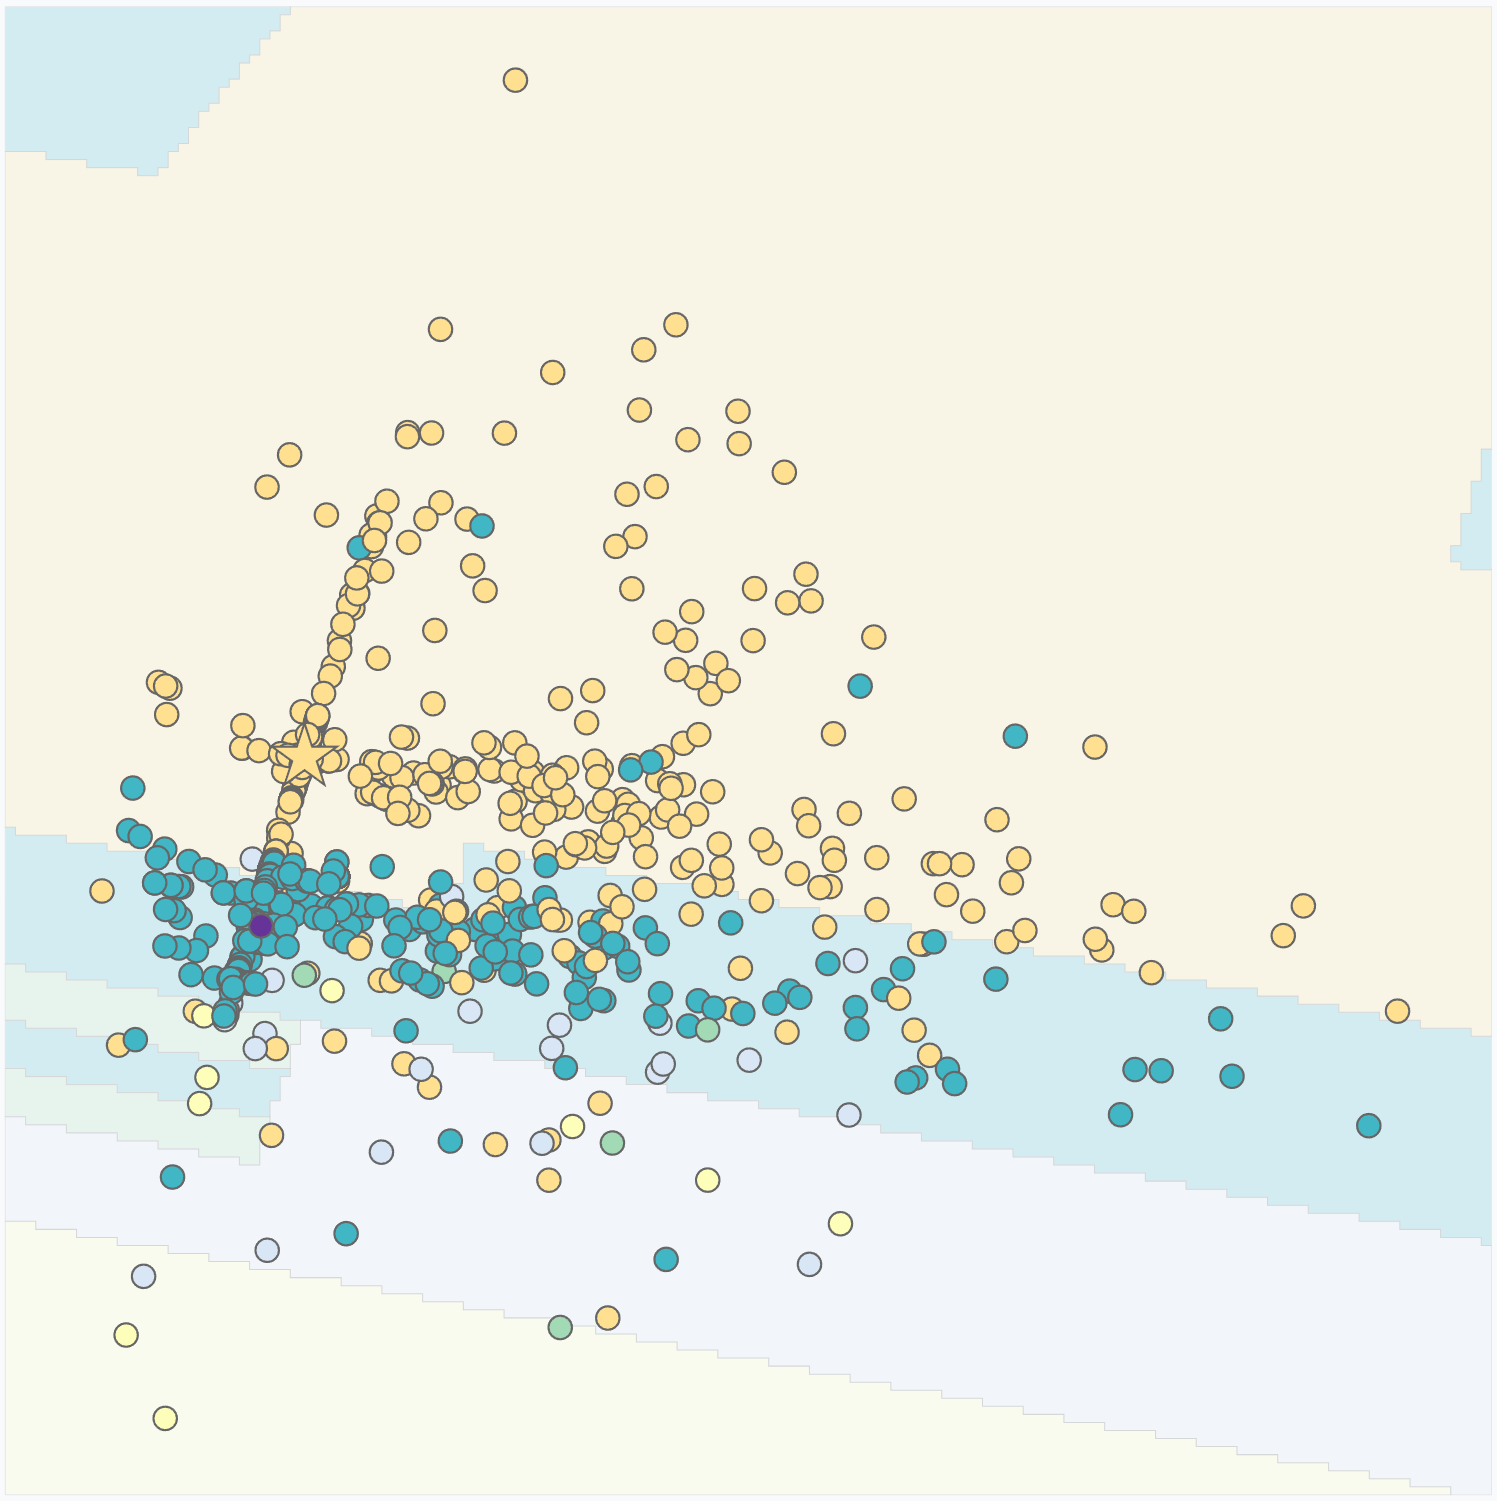
\includegraphics[width=\textwidth,height=0.4\textheight,keepaspectratio]{images/ds_interaction_p3_highlight_scatter.png}
        \caption{PCA scatter plot with highlighted percentile\_3 instance}
        \label{fig:ds_interaction_p3_highlight_scatter}
    \end{subfigure}
    \hfill
    \begin{subfigure}[c]{0.48\textwidth}
        \centering
        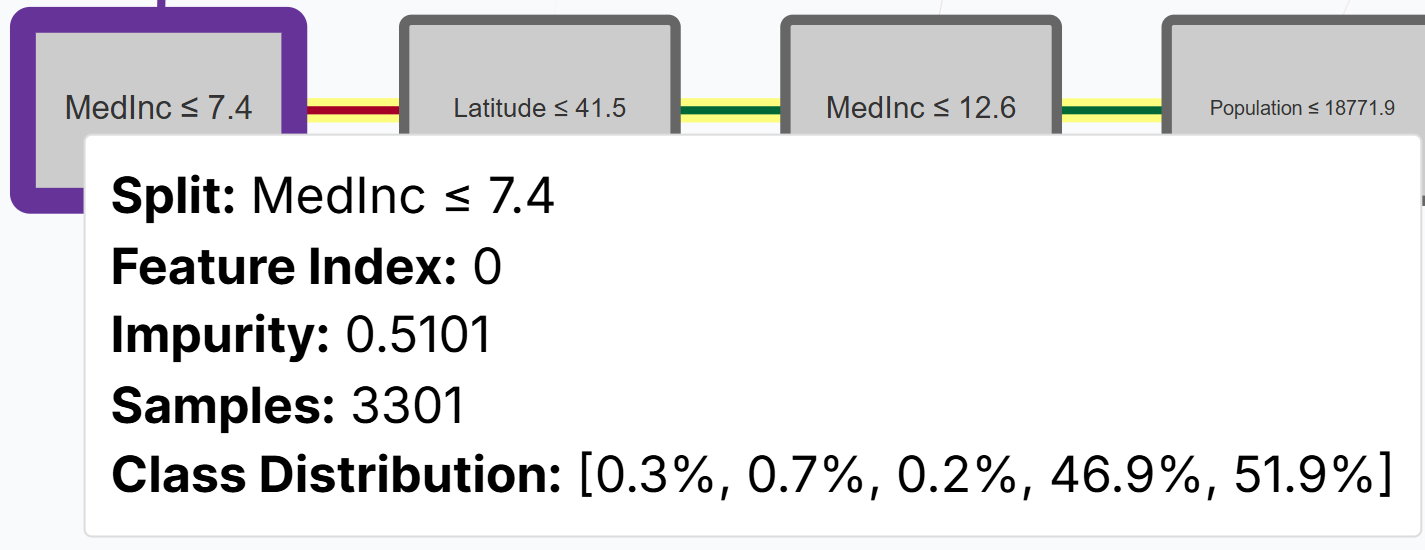
\includegraphics[width=\textwidth,height=0.4\textheight,keepaspectratio]{images/ds_interaction_p3_highlight_tree_top.png}
        \caption{Tree visualization top section showing root split}
        \label{fig:ds_interaction_p3_highlight_tree_top}
    \end{subfigure}
    
    \vspace{0.5cm}
    
    \begin{subfigure}[c]{0.48\textwidth}
        \centering
        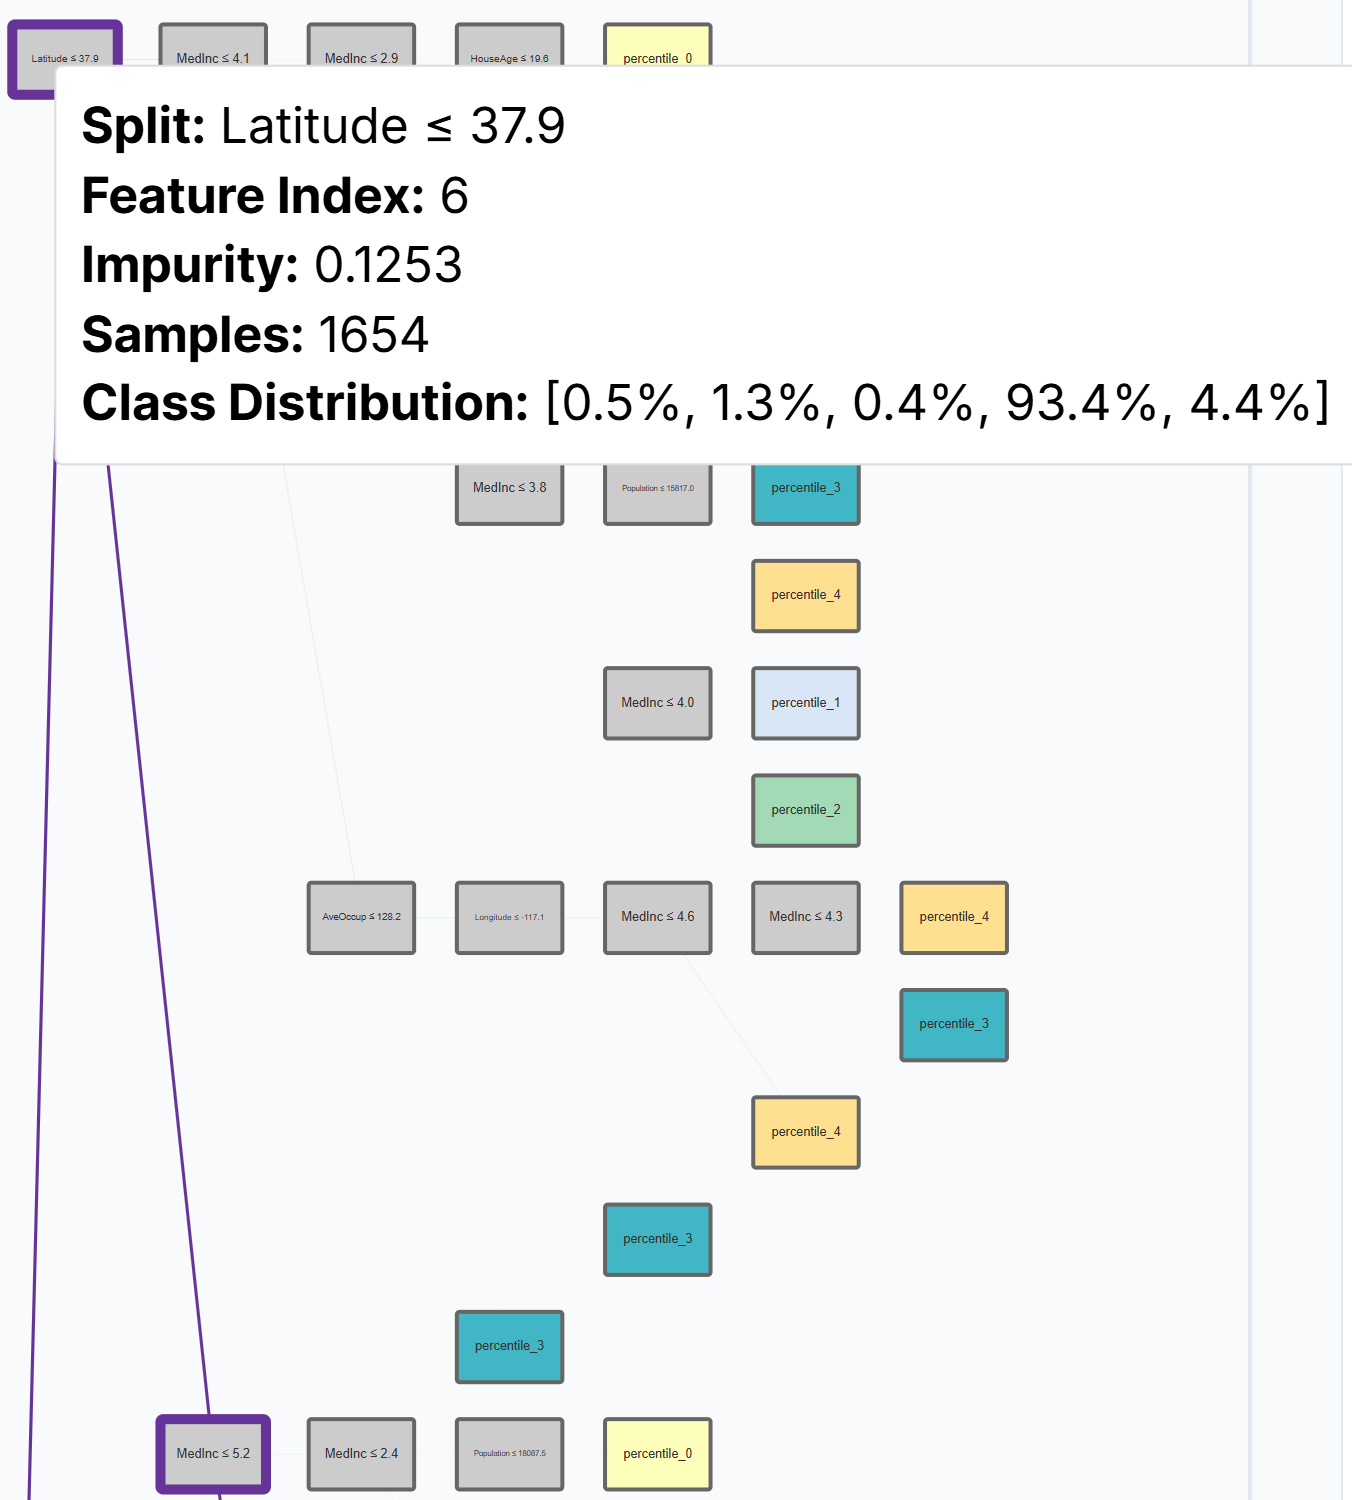
\includegraphics[width=\textwidth,height=0.4\textheight,keepaspectratio]{images/ds_interaction_p3_highlight_tree_mid.png}
        \caption{Tree visualization middle section with highlighted path}
        \label{fig:ds_interaction_p3_highlight_tree_mid}
    \end{subfigure}
    \hfill
    \begin{subfigure}[c]{0.48\textwidth}
        \centering
        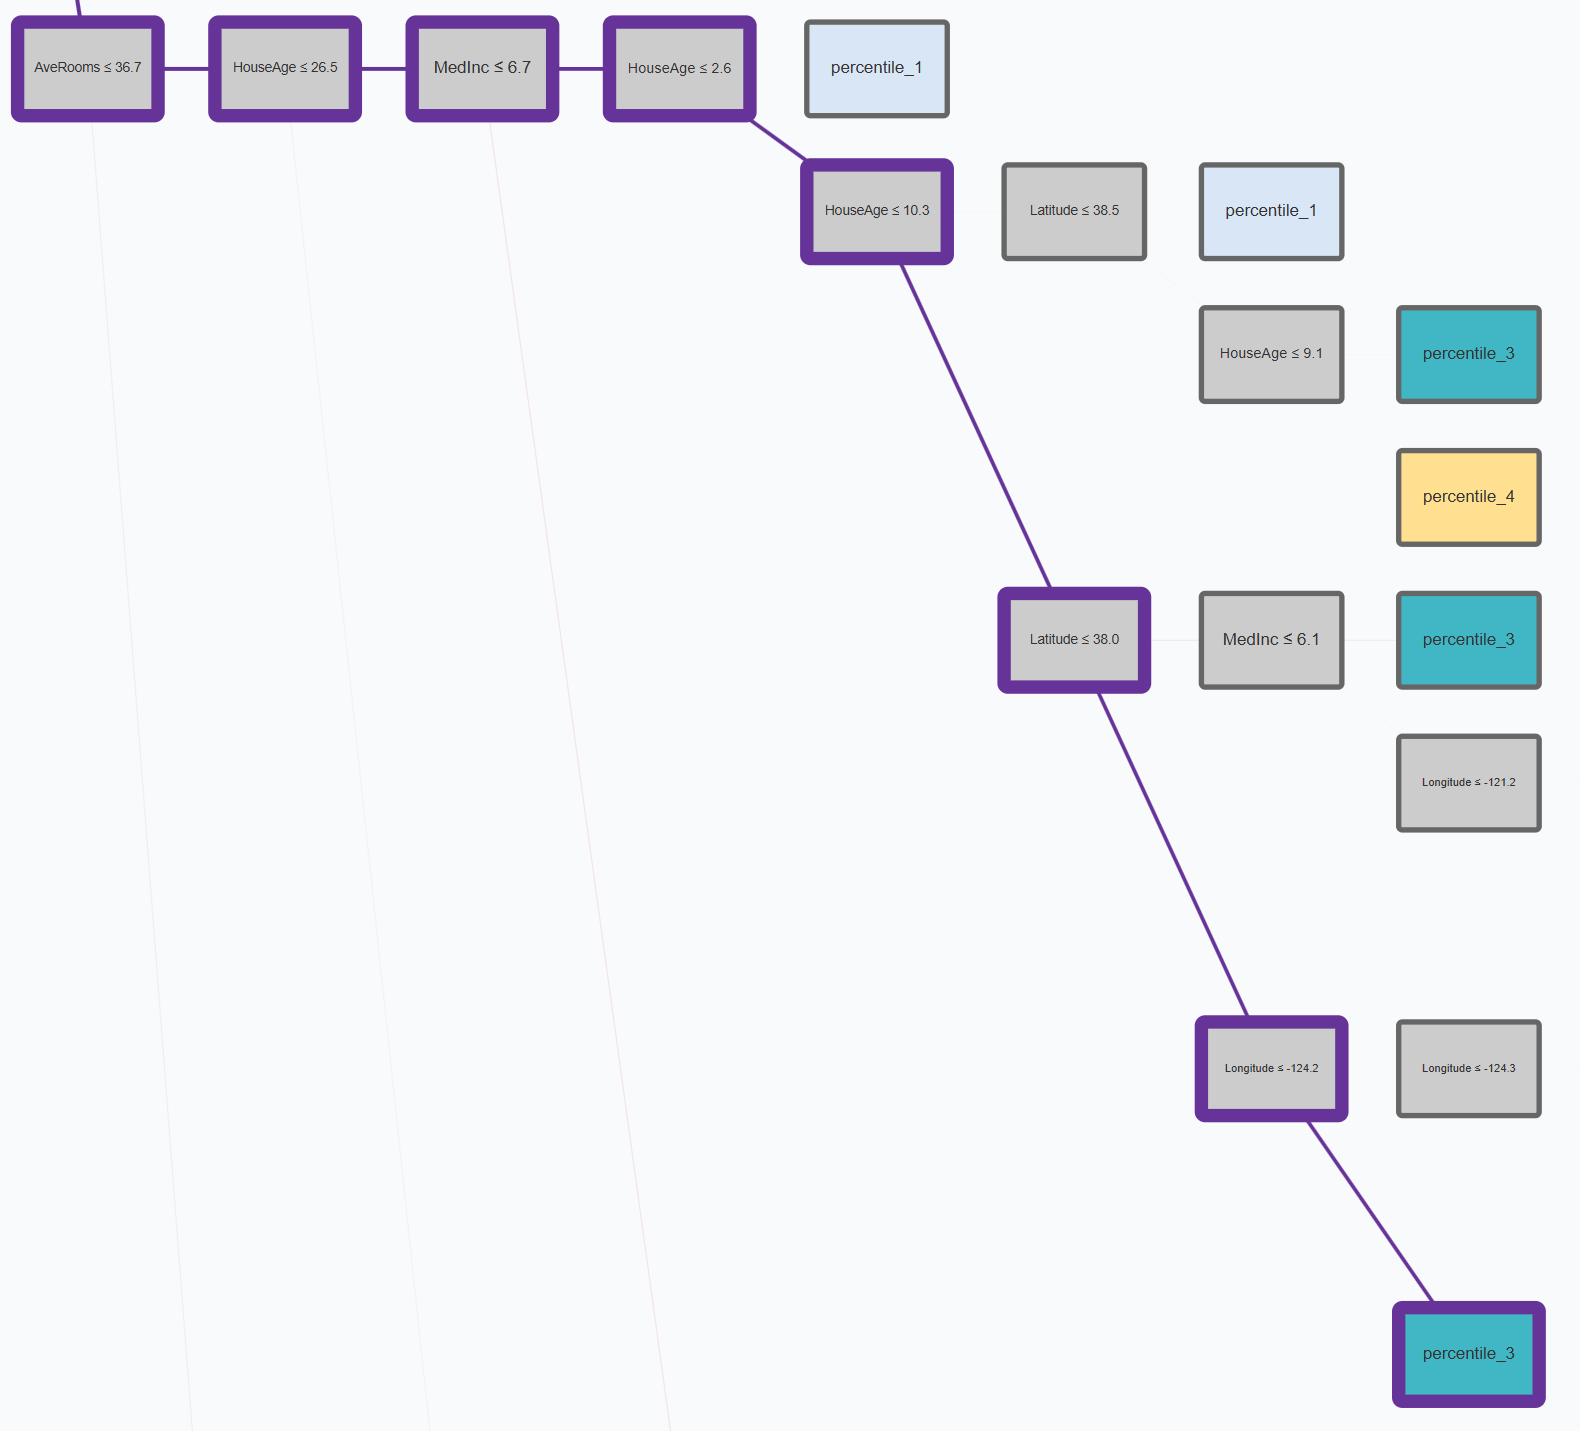
\includegraphics[width=\textwidth,height=0.4\textheight,keepaspectratio]{images/ds_interaction_p3_highlight_tree_bottom.png}
        \caption{Tree visualization bottom section showing path to and percentile\_3 leaf node}
        \label{fig:ds_interaction_p3_highlight_tree_bottom}
    \end{subfigure}
    \caption{Coordinated visualization interaction: clicking a percentile\_3 instance in the PCA scatter plot (a) triggers path highlighting across the full tree visualization (b-d), demonstrating bidirectional coordination between spatial and symbolic representations with detailed view of split conditions}
    \label{fig:ds_interaction_p3_highlight}
\end{figure}


The data scientist makes use of the coordinated visualizations to explore the relationship between neighborhood instances and their decision paths. They begin by selecting a percentile\_3 instance near the class boundary in the PCA scatter plot (Figure \ref{fig:ds_scatter_pca_3000}).

Figure \ref{fig:ds_interaction_p3_highlight} captures this coordinated highlighting. The selected point in the scatter plot appears in the highlight color, and emphasis is put on the tree path from root to the corresponding leaf. This immediate visual feedback confirms the logical conditions that led to this specific instance's classification.

The data scientist hovers over the percentile\_3 leaf node in the tree to examine detailed statistics. The tooltip reveals that around 1400 instances from the 3,000-instance neighborhood follow this path. This substantial sample count indicates a robust, stable pattern rather than an isolated edge case.

The data scientist systematically explores instances across different regions of the scatter plots. They click on a percentile\_0 instance located in the peripheral region of the PCA projection, interaction shown in Figure \ref{fig:ds_scatter_pca_3000}. The tree highlighting reveals a long path through multiple splits, ultimately reaching a small leaf node with only a few instances. This scarce population contrasts sharply with the number of instances for the percentile\_3 counterfactual rule leaf and the heavily populated percentile\_4 rule leaf. The data scientist recognizes that rules based on such small sample counts carry lower confidence—they may represent genuine but rare decision patterns.

They switch between the three tree visualization layouts (Tree Layout, Rule and Counterfactual Rules Centered, Rule Centered) to examine the same highlighted path from different visual perspectives. The Tree Layout provides an overview of the entire decision structure. The Rule and Counterfactual Rules Centered view positions the explained instance's path at the bottom, facilitating comparison between the factual rule and alternative paths. The Rule Centered view collapses irrelevant subtrees, focusing attention on the paths most relevant to understanding the explained instance. Each layout offers distinct advantages for different analytical tasks.

Throughout this interactive exploration, the data scientist builds comprehensive understanding by iteratively forming hypotheses, testing them through instance selection, and observing the corresponding tree paths and tooltip information. The bidirectional coordination proves essential: scatter plot interactions reveal rule structures, while tree interactions reveal instance distributions.

\subsection{Validating Generality: Middle-Class Instance Analysis}

After completing the analysis of the percentile\_4 instance, the data scientist reflects on whether the instance selection influenced the genetic algorithm's exploration behavior. The initial instance belonged to percentile\_4, representing properties at the upper boundary of the dataset's price distribution. The data scientist hypothesizes that this extreme position might have constrained the genetic algorithm's ability to explore diverse regions of the feature space, biasing the observed patterns and consequential understanding of the model toward only high-value property characteristics.

To validate whether the explanation patterns generalize across different regions of the decision space, they select a new instance from percentile\_2, the middle class of the five-category distribution. This instance represents properties with moderate prices (\$157,300-\$209,400), occupying the central region of the price distribution rather than an extreme. The selected percentile\_2 instance has median income \$338,410, house age 29 years, 4.8 average rooms, 1.002 average bedrooms, population 1919, average occupancy 2.7, located at latitude 37.69 and longitude -121.76 (East Bay area, near Livermore).

The data scientist generates explanations for this percentile\_2 instance using both 500 and 3,000 synthetic neighbors to examine whether the neighborhood size effects observed for the percentile\_4 instance hold for instances in different regions of the decision space.

The analysis reveals patterns remarkably consistent with the percentile\_4 case. The UMAP projection for the 500-instance neighborhood, shown in Figure \ref{fig:ds_p2_scatter_umap_500}, displays a clusters of percentile\_2 (\#a1dab4) instances, surrounding the explained instance, and another cluster of percentile\_1 (\#D9E6F5) instances. Other percentiles appear throughout the projection, and overall the spatial distribution patterns are similar to those observed in the percentile\_4 analysis. The genetic algorithm again focuses exploration on the local decision space around the explained instance, generating synthetic neighbors primarily within the predicted class region and its immediate boundaries.

The surrogate tree structure maintains the same fundamental pattern observed previously: one clear factual rule path leading to the predicted class (percentile\_2), and one meaningful counterfactual rule. The counterfactual rule in this case leads to percentile\_1 rather than percentile\_3, reflecting the downward rather than upward class transition relevant for a middle-range instance. 

When the data scientist regenerates the explanation with 3,000 synthetic instances, the patterns again parallel the previous analysis. The PCA projection with decision boundaries, shown in Figure \ref{fig:ds_p2_scatter_pca_3000}, reveals increased instance density and clearer boundary visualization. The decision space appears slightly more mixed compared to the percentile\_4 case. This reflects the genuine decision landscape for middle-range properties, which naturally have adjacent class boundaries on both sides rather than the more isolated position of extreme-value properties.

\begin{figure}[ht]
\centering
\begin{subfigure}[c]{0.48\textwidth}
    \centering
    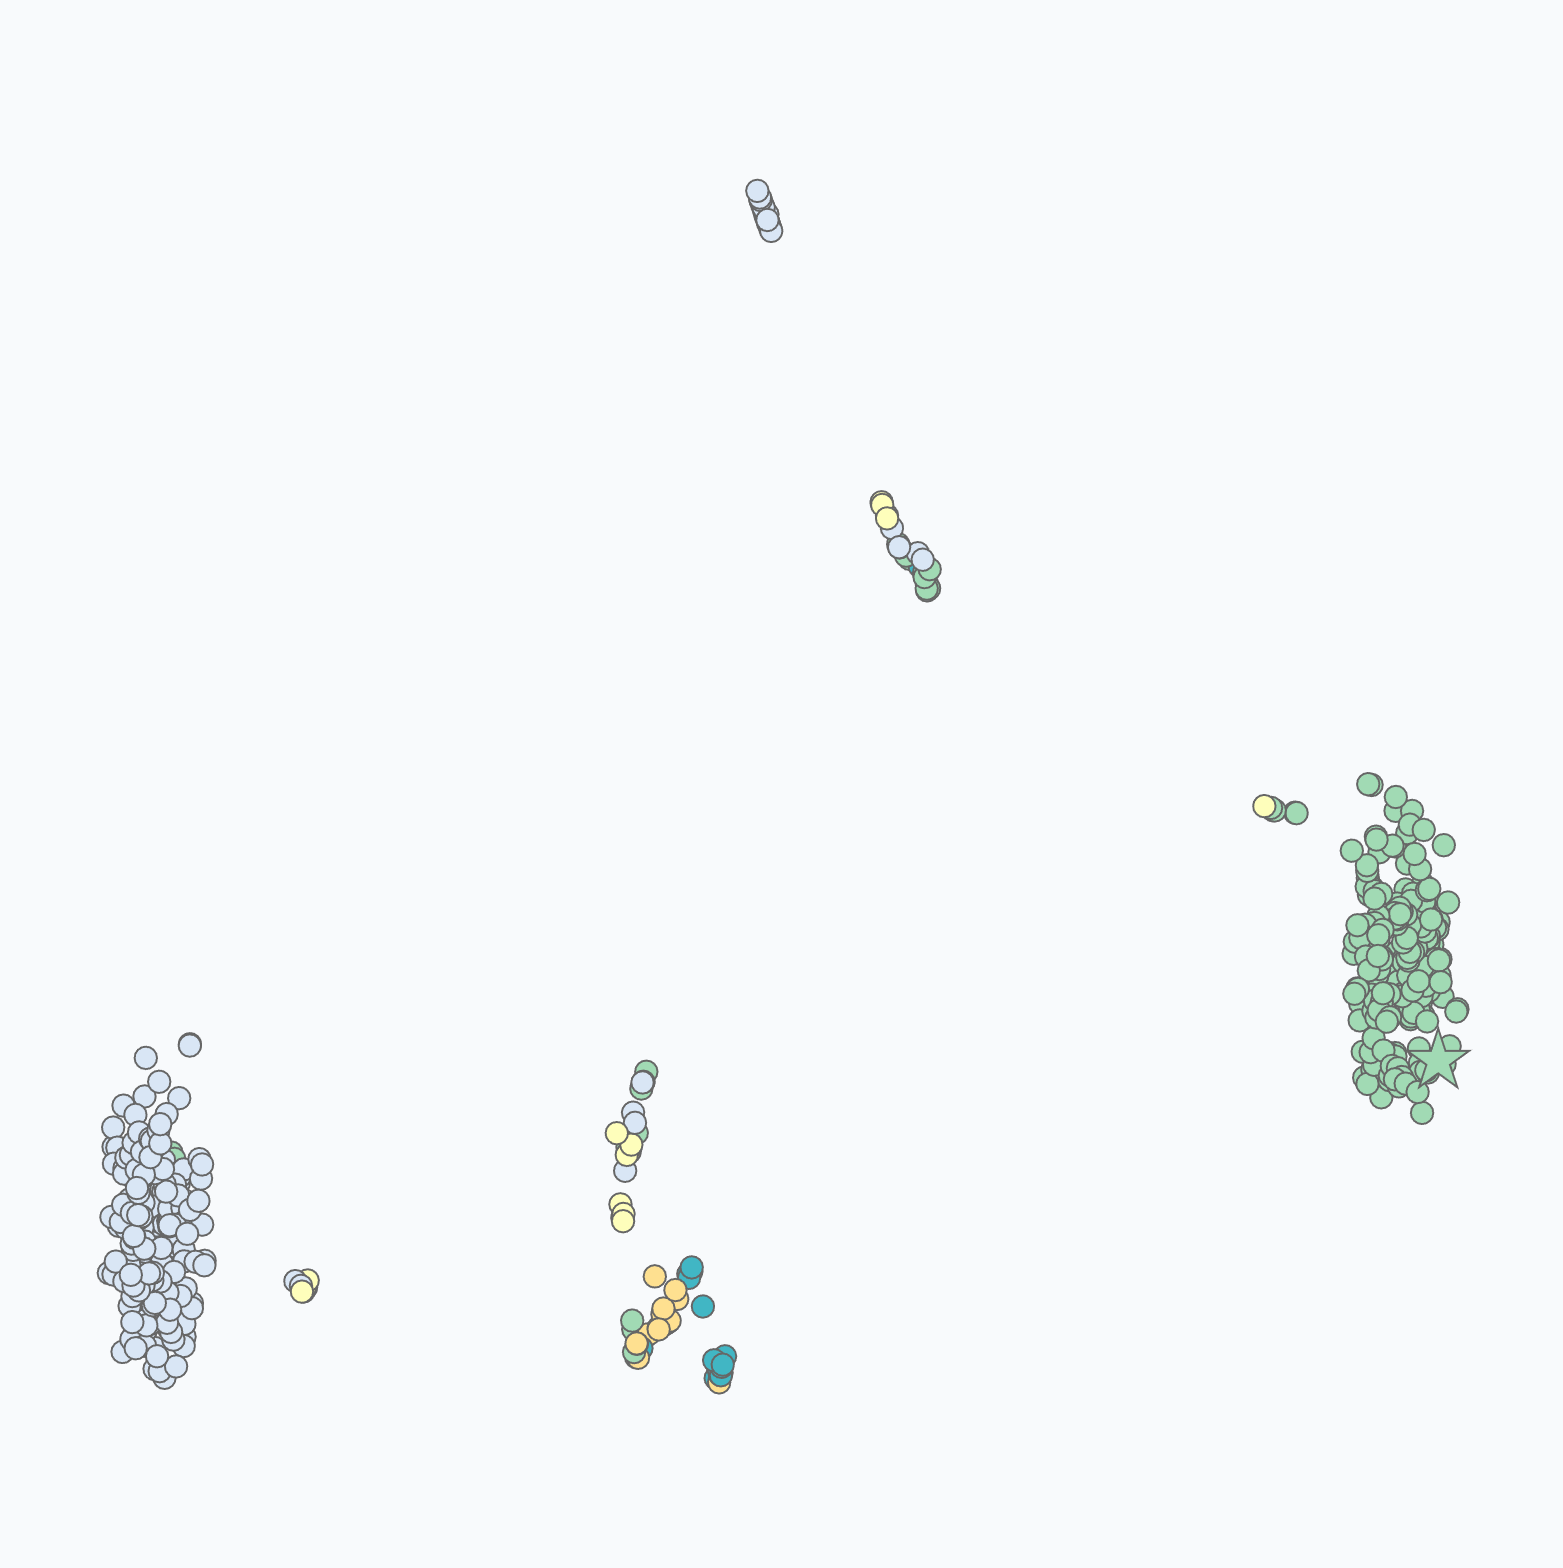
\includegraphics[width=\textwidth]{images/ds_p2_scatter_umap_500.png}
    \caption{UMAP projection of 500-instance synthetic neighborhood showing cluster structures similar to percentile\_4 analysis with dominant predicted class and counterfactual rule cluster, plus scattered adjacent class instances}
    \label{fig:ds_p2_scatter_umap_500}
\end{subfigure}
\hfill
\begin{subfigure}[c]{0.48\textwidth}
    \centering
    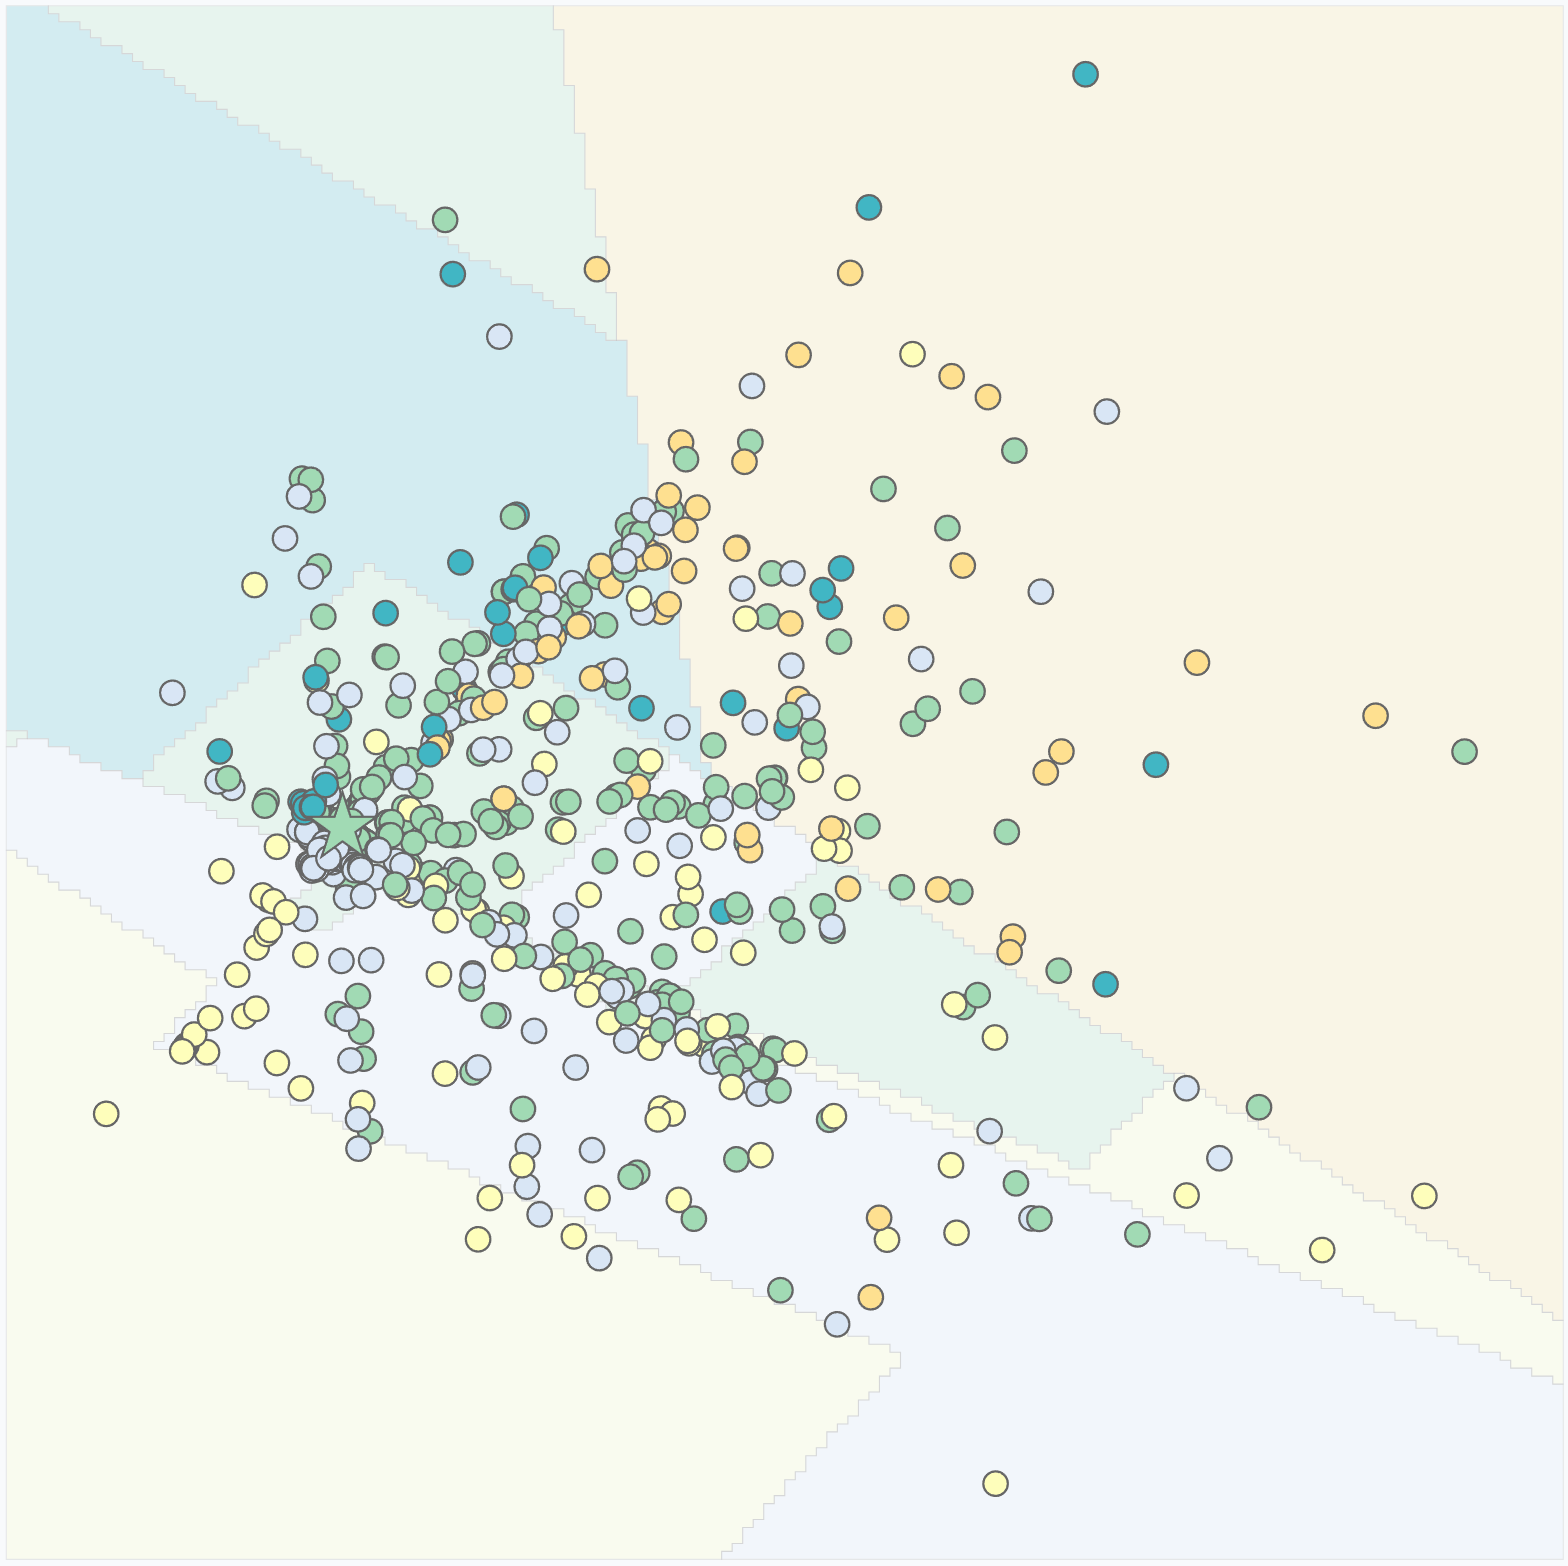
\includegraphics[width=\textwidth]{images/ds_p2_scatter_pca_3000.png}
    \caption{PCA projection with decision boundaries for 3000-instance neighborhood showing slightly more mixed decision space with adjacent class regions visible on multiple sides of the predicted class region}
    \label{fig:ds_p2_scatter_pca_3000}
\end{subfigure}
\caption{Comparison of UMAP and PCA projections for percentile\_2 instance neighborhoods at different scales}
\label{fig:ds_p2_projections}
\end{figure}

The expanded neighborhood yields a refined factual rule with additional conditions, maintaining the same refinement pattern observed in the percentile\_4 analysis. 
This validation analysis confirms that the explanation methodology produces consistent, stable results across different regions of the decision space. 
The slightly more mixed decision space for the percentile\_2 instance reflects genuine classifier behavior rather than algorithm limitation, accurately characterizing the more complex boundary structure surrounding middle-range properties.

\subsection{Insights and Methodological Implications}

Through this analysis, the data scientist derives several key insights about the Random Forest classifier's behavior on the California Housing task. They confirm that geographic location (Latitude in particular) serves as a secondary decision factor, with the approximate boundary at 37.5 degrees latitude corresponding to the transition from Bay Area premium pricing to lower-cost regions. They identify MedInc as the most critical feature, with thresholds around \$730,000 separating high-value properties from lower-value ones. The dual MedInc conditions in the refined 3000 samples rule further reveal that typical high-value properties occupy a specific income range (\$740,000-\$1,260,000) rather than simply exceeding a lower threshold.

The data scientist recognizes that neighborhood size critically affects explanation detail and confidence. The 500-instance default proves adequate for understanding the explained instance's immediate classification and captures the primary counterfactual scenario (percentile\_3). The simpler rule extracted from the 500-instance neighborhood provides clear, interpretable logic that stakeholders can readily understand. The 3,000-instance neighborhood provides substantially more comprehensive coverage, revealing additional counterfactual rules for all five price percentiles and enabling extraction of refined rules with multiple conditions that capture secondary decision factors. The more complex rules from the larger neighborhood offer deeper insight but require more careful interpretation.

This experience informs their approach to future model explanation tasks. They establish a workflow principle: begin with default parameters for rapid initial exploration, but systematically increase neighborhood size when dealing with multi-class problems or when initial explanations appear incomplete. They also recognize the value of comparing multiple neighborhood sizes to validate explanation consistency and identify potential artifacts of insufficient sampling.

The interactive visualization proves essential for this analytical workflow. The ability to rapidly switch between different dimensionality reduction methods (UMAP for cluster structure, PCA for boundaries), explore tree structures at multiple levels of detail through three alternative layouts, and confirm patterns through coordinated highlighting provides flexibility that enables thorough analysis. The coordinated interaction between scatter plots and tree visualizations allows the data scientist to continuously validate rules against actual instance distributions, building confidence in the extracted explanations.